%!TEX root = ../dokumentation.tex

\section{Anfänglicher Projektstand}
Das \textbf{Find your Camp} Projekt, befasst sich mit der Entwicklung einer Smartphoneanwendung für Androidgeräte, als Verleihsystem von privaten Grundstücken als Unterkunft. Die erste Projektphase befasste sich dabei mit der Entwicklung eines Exposes und anschließender Konzepterarbeitung zur Ausgangsidee. Im Rahmen dieser Phase wurden vorhandene Alternativen am Markt untersucht, Alleinstellungsmerkmale und Risiken in Bezug auf die Anwendungsdomäne abgewogen und es fand eine thematische Einarbeitung in die Problemdomäne statt.\\
Der Beschäftigung mit MCI Aspekten folgte der Entschluss, das Vorgehen auf Basis des \textbf{Usage Centered Design} durchzuführen, da der Schwerpunkt des Projektes auf den Interaktionen der Anwender liegt und die erwartete Benutzergruppe nicht durch bestimmte Merkmale konkretisiert werden kann.\footnote{Konzeptseite 12}
Weiterhin fanden erste Auseinandersetzungen mit dem Nutzungskontext\footnote{ab Konzeptseite 18}, der Nutzungsmotivation und ersten Anforderungsanalysen statt.\\
Für die Umsetzung wurde eine Systemarchitektur unter Einbezug der Google Cloud angedacht und die erste Testphase über die Proof-of-Concepts\footnote{Konzeptseite 41} geplant.\\

Zur weiteren Projektephase wurden zudem 2 Meilensteine definiert. Die Bearbeitung des ersten Meilensteins, sah die Umsetzung der weiteren MCI Methoden und die Durchführung der Proof-of-Concepts vor, wie dem Auszug des Projektplans (Abb. \ref{fig:projektplan}) bei Konzeptabgabe zu entnehmen ist. Angedacht waren hierfür 3 Wochen Arbeitszeit, deren einzelnen Schritte nach und nach verfeinert werden.
\begin{figure}[H]
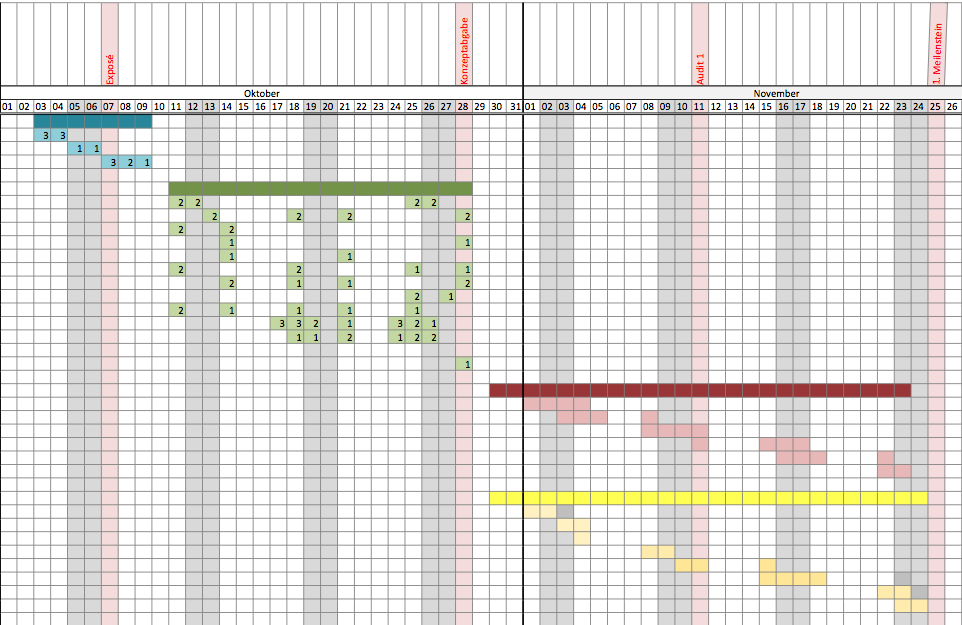
\includegraphics[width=1\textwidth]{./images/ausgangsplan.png}
\caption{Ausgangsplan bei Konzeptabgabe}
\label{fig:projektplan}
\end{figure}

Innerhalb welcher Zeitrahmen die einzelnen Arbeitsschritte letztendlich umgesetzt wurden, wird an gegeben Stellen deutlich gemacht.\\

\subsection{Konzeptüberarbeitungen}
Bevor mit der Dokumentation neuer Ergebnisse begonnen wurde, ging es um die Umsetzung des Konzeptfeedbacks und die Überarbeitung vorhandener Ausarbeitungen.\\
Damit die einzelnen Abschnitte inhaltlich etwas deutlicher aufeinander aufbauen, wurde die grundlegende Struktur des Dokumentes überarbeitet und das Geschäftsmodell sowie Zielhierachie als eigener Schwerpunkt herausgenommen. Die Abwägung des MCI Vorgehens wurde erweitert und an geeigneten Stellen präziser formuliert.\\

Erste Ansätze zum Geschäftsmodell wurden konkretisiert und mit Kennzahlen versehen. Die Vorgehensmöglichkeiten wurden dabei im Gespräch abgewogen und zu einem einheitlichen Modell zusammengefasst, anhand dessen eine Finanzierung als möglich erachtet wird. Die Zielhierachie wurde genauer auf das Projekt bezogen, da der vorherige Fokus zu wirtschaftlich und von langfristigen Zielen geprägt war.

\newpage
Ansätze zur Risikominimierung wurden ausführlicher und mit deutlicherem Bezug zum Konzept dokumentiert. Innherhalb der Anforderungsanalyse wurden nach eigenem Ermessen die funktionalen und qualitativen Anforderungen ausgebaut und zusätzlich erste organisatorische Anforderungen betrachtet.\\
Im WBA2 Teil, wurde das Kapitel zum Datenmodell erarbeitet und angedachte Proof-of-Concepts mit Bedeutung für das System genauer in Zusammenhang gebracht.\\

Für die Überarbeitung genannter Punkte, wurden im Vorfeld 1-2 weitere Arbeitstag eingeplant. Die letztendliche Arbeitszeit erstreckte sich jedoch auf eine gesamte Woche, was zur Folge hatte, dass der angesetzte Zeitrahmen der MCI Bearbeitungen verschoben werden musste. Der Grund der Überarbeitungsdauer liegt vor allem an der Bearbeitungstiefe, da gesamtes Konzept geprüft und wesentliche Aspekte weiter ausgearbeitet wurden. Kritisch für den Zeitplan wurde dies jedoch nicht angesehen, da die Überarbeitung auch Ergänzungen beinhaltet, die an anderer Stelle während der Dokumentation aufgetreten wären, jetzt jedoch im Konzept Einzug fanden.\\ Mit fortschreitender Projektzeit wurde deutlich, dass der erste gesetzte Meilenstein, bezogen auf die MCI Auseinandersetzung, mehr einer ersten Iterationsphase gleich kommt, als einer ausreichenden Betrachtung. Aufgrund des iterativen Charakters eines menschbezogenen Entwicklungsprojekts mit Evaluationen und Überarbeitungen der Ergebnisse, wurde die MCI Betrachtung über den gesamten Projektverlauf ausgelegt.

